\documentclass[12pt,a4paper]{article}
\title{Plantilla}
\usepackage{UPIITA}
\asignatura{Diseño y analisis de algoritmos}
\carrera{MCC}
\titulo{Practica 1: Emparejamiento Estable}
\alumno{Ronquillo Núñez Braulio Alberto}
\profesor{Raul Acosta Bermejo}
\begin{document}
\maketitlepage % Portada

%\tableofcontents %Índice
%\newpage
%\listoffigures   %Índice de figuras
%\newpage        
%\listoftables   %Índice de tablas

% Cuerpo del Documento
%\newpage

% Insertar .tex al documento
\newpage
\fontsize{10pt}{12pt}\selectfont
\twocolumn
\section{Introducción}

El Problema de Emparejamiento Estable (Stable Matching Problem) fue formalizado por Gale y Shapley en 1962 \cite{gale_shapley_1962}. El problema consiste en emparejar dos conjuntos disjuntos de igual tamaño, donde cada participante posee un orden completo de preferencias sobre los elementos del conjunto opuesto. El objetivo es encontrar un emparejamiento que sea estable.

Un emparejamiento es estable si no existe un par bloqueante, es decir, un par de participantes que prefieran estar emparejados entre sí antes que con sus respectivas parejas asignadas. La estabilidad garantiza que ningún par tenga incentivos para desviarse del resultado obtenido.

El algoritmo de Aceptación Diferida propuesto por Gale y Shapley garantiza la existencia de al menos un emparejamiento estable para cualquier instancia válida del problema \cite{gale_shapley_1962}. Desde el punto de vista computacional, este algoritmo tiene complejidad temporal $O(N^2)$ en el peor caso \cite{gusfield_irving_1989}, ya que cada participante puede realizar a lo sumo $N$ propuestas.

El problema tiene aplicaciones relevantes en diseño de mecanismos y asignación de recursos, como en sistemas de residencias médicas y mercados laborales \cite{roth_vande_1990}. En esta práctica se implementa el algoritmo de Gale--Shapley considerando ambas variantes posibles (cuando propone cada conjunto) y se analiza experimentalmente su comportamiento temporal.

\subsection{Objetivos}
El objetivo general de esta práctica es implementar y evaluar experimentalmente el algoritmo de Gale--Shapley para resolver el Problema de Emparejamiento Estable en su versión básica, considerando dos conjuntos de igual cardinalidad $N$ y listas completas de preferencias.

De manera específica, se busca:
\begin{itemize}
    \item modelar correctamente una instancia del SMP a partir de dos conjuntos disjuntos con preferencias completas;
    \item implementar el algoritmo de Gale--Shapley de forma que pueda ejecutarse en ambas variantes: cuando el primer conjunto realiza las propuestas y cuando las realiza el segundo;
    \item medir el tiempo asociado al proceso de emparejamiento para diferentes tamaños de entrada, con el fin de observar cómo cambia el costo computacional conforme crece $N$;
    \item contrastar los resultados experimentales con la complejidad teórica $O(N^2)$ reportada para el algoritmo;
    \item interpretar los resultados obtenidos y verificar si el comportamiento observado es consistente con la teoría revisada.
\end{itemize}

\section{Metodologia}
La metodología empleada en esta práctica consistió en implementar el algoritmo de Gale--Shapley para resolver el Problema de Emparejamiento Estable y, posteriormente, evaluar experimentalmente su comportamiento temporal para distintos tamaños de entrada.

En una primera etapa se desarrolló una implementación eficiente del algoritmo considerando ambas variantes posibles: cuando el conjunto de hombres realiza las propuestas y cuando el conjunto de mujeres lo hace. Para optimizar el desempeño, se utilizó un esquema de \textit{ranking inverso} que permite comparar preferencias en tiempo constante $O(1)$, evitando recorridos lineales en las listas de preferencias.

En una segunda etapa se generaron automáticamente instancias de entrada para valores crecientes de $N$. Cada instancia contiene dos conjuntos de tamaño $N$ con listas completas de preferencias generadas aleatoriamente. La generación de datos se automatizó mediante un script independiente, lo que permitió controlar de manera sistemática el tamaño de las entradas y construir un conjunto de pruebas homogéneo.

Posteriormente, para cada instancia generada, se ejecutó el algoritmo y se registró el tiempo correspondiente al proceso de emparejamiento. Aunque en una implementación completa pueden distinguirse las fases de lectura, procesamiento e impresión, en este análisis se aisló el tiempo del algoritmo principal para que la medición reflejara de forma más precisa el costo computacional del procedimiento de Gale--Shapley.

Las mediciones se realizaron utilizando un temporizador de alta resolución (\texttt{perf\_counter}) y los resultados fueron almacenados en una tabla estructurada que relaciona el tamaño $N$ con el tiempo correspondiente.

Finalmente, los tiempos obtenidos fueron graficados utilizando tanto escala lineal como escala logarítmica para el eje de $N$, con el objetivo de analizar la forma del crecimiento temporal y contrastarlo con la complejidad teórica $O(N^2)$.

\subsection{Herramientas}

Para el desarrollo de la práctica se utilizaron las siguientes herramientas:

\begin{itemize}
    \item Lenguaje de programación Python 3 para la implementación del algoritmo y generación de instancias.
    \item Bibliotecas estándar de Python para medición de tiempos y manejo de estructuras de datos.
    \item Biblioteca \texttt{matplotlib} para la generación de gráficas.
    \item Entorno de desarrollo local y sistema de control de versiones Git para organización del código.
\end{itemize}

\section{Resultados}

Para evaluar el comportamiento temporal del algoritmo de Gale--Shapley se trabajó con instancias de entrada de tamaños crecientes $N$, desde $32$ hasta $2000$. Para cada valor de $N$ se ejecutó el procedimiento de emparejamiento y se registró el tiempo necesario para realizar únicamente esa fase del proceso, con el fin de centrar el análisis en el costo del algoritmo y no en operaciones auxiliares como la lectura o la impresión.

La Tabla~\ref{tabla:tiempos} muestra los tiempos obtenidos para distintos valores de $N$.

\begin{table}[h]
\centering
\caption{Tiempos de ejecución del algoritmo de Gale--Shapley}
\label{tabla:tiempos}
\begin{tabular}{|c|c|}
\hline
\textbf{N} & \textbf{Tiempo (ms)} \\
\hline
32   & 0.255 \\
64   & 0.694 \\
128  & 2.317 \\
256  & 10.178 \\
384  & 24.806 \\
512  & 41.967 \\
640  & 62.640 \\
768  & 89.410 \\
896  & 119.286 \\
1024 & 215.997 \\
1200 & 220.035 \\
1400 & 332.430 \\
1600 & 405.424 \\
1800 & 532.750 \\
1900 & 586.778 \\
2000 & 646.559 \\
\hline
\end{tabular}
\end{table}

Los datos muestran una tendencia creciente en el tiempo de ejecución conforme aumenta el tamaño de entrada. Por ejemplo, para $N=32$ el tiempo medido fue de $0.255$ ms, mientras que para $N=2000$ se registró un tiempo de $646.559$ ms. Esta diferencia evidencia que el costo del algoritmo aumenta de manera importante al incrementar la dimensión del problema.

Con base en estos resultados se generaron gráficas utilizando escala lineal y escala logarítmica para el eje de $N$, tal como se recomienda en el enunciado de la práctica. La gráfica en escala lineal permite observar con claridad el crecimiento acelerado del tiempo de ejecución, mientras que la representación log-log facilita contrastar el comportamiento observado con un modelo polinómico.
\subsection{Análisis de resultados}

La Figura~\ref{fig:lineal} muestra el tiempo de ejecución del algoritmo en función del tamaño de entrada $N$ en escala lineal. Se observa que el crecimiento no es lineal, sino que aumenta de manera acelerada conforme $N$ se incrementa. Este comportamiento es consistente con una complejidad mayor que $O(N)$.

\begin{figure}[h]
\centering
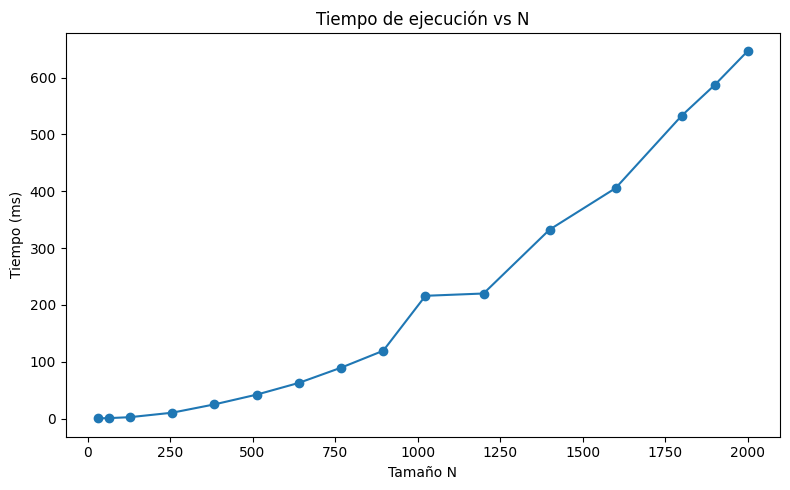
\includegraphics[width=\columnwidth]{figuras/grafica_lineal.png}
\caption{Tiempo de ejecución en escala lineal.}
\label{fig:lineal}
\end{figure}

Para analizar el comportamiento asintótico con mayor claridad, se utilizó una representación log-log, mostrada en la Figura~\ref{fig:loglog}. En esta escala, si el comportamiento sigue una ley polinómica $T(N) = cN^k$, los datos deben aproximarse a una recta cuya pendiente corresponde al exponente $k$.

\begin{figure}[h]
\centering
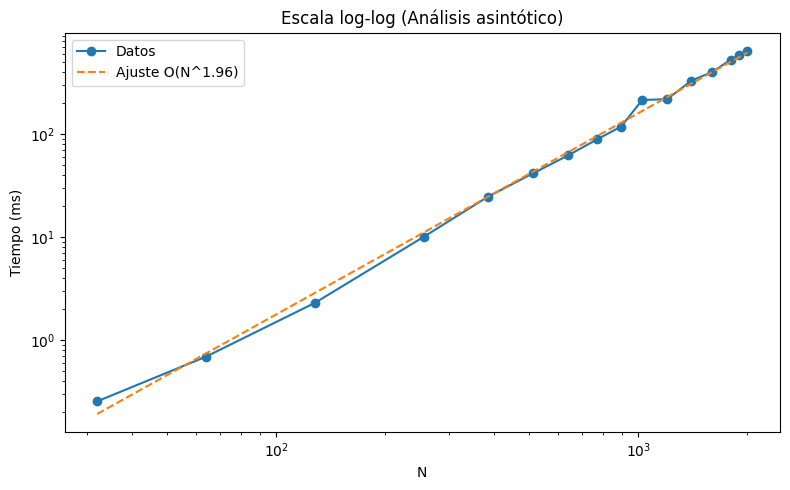
\includegraphics[width=\columnwidth]{figuras/grafica_loglog.png}
\caption{Tiempo de ejecución en escala log-log.}
\label{fig:loglog}
\end{figure}

El ajuste realizado sobre los datos experimentales produjo una pendiente aproximada de $k \approx 1.96$, valor muy cercano al exponente teórico esperado $k = 2$. En consecuencia, los resultados experimentales respaldan que el algoritmo de Gale--Shapley presenta un comportamiento cuadrático $O(N^2)$ en el peor caso. Además, el ajuste obtenido muestra una alta concordancia con la tendencia observada en los datos, por lo que la interpretación no depende de un punto aislado, sino del comportamiento global de la curva.

Las pequeñas desviaciones observadas respecto al ajuste teórico pueden atribuirse a factores propios del entorno de ejecución, como la administración de memoria, la caché del procesador y la sobrecarga del sistema operativo. Por ejemplo, algunos incrementos entre tamaños consecutivos no siguen una proporción exactamente uniforme; sin embargo, estas variaciones locales no modifican la tendencia general de crecimiento.

\subsection{Observaciones}

Los resultados permiten afirmar que la implementación cumple con el comportamiento esperado para este problema. A medida que $N$ crece, el número de propuestas potenciales también aumenta y, por ello, el tiempo de ejecución se incrementa de manera compatible con una función cuadrática.

Asimismo, debe considerarse que las mediciones dependen del entorno experimental y de la instancia utilizada para cada tamaño. Por esta razón, pequeñas fluctuaciones entre valores consecutivos son normales y no contradicen la complejidad teórica del algoritmo. En conjunto, la tabla y las gráficas aportan evidencia suficiente para sostener que la implementación reproduce el desempeño asintótico esperado para Gale--Shapley.

\section{Conclusiones}

En esta práctica se implementó el algoritmo de Gale--Shapley para resolver el Problema de Emparejamiento Estable y se evaluó experimentalmente su comportamiento temporal para distintos tamaños de entrada. Con ello, se cumplió el objetivo principal de analizar cómo evoluciona el costo computacional del algoritmo conforme aumenta el valor de $N$.

Los resultados obtenidos muestran que el tiempo de ejecución crece de manera aproximadamente cuadrática con respecto a $N$. El ajuste realizado en escala log-log arrojó una pendiente cercana a $1.96$, valor consistente con la complejidad teórica $O(N^2)$ del algoritmo en el peor caso. Por lo tanto, el análisis empírico concuerda con lo establecido en la literatura para el algoritmo de Gale--Shapley.

Las variaciones observadas entre los datos experimentales y el modelo ideal pueden explicarse por factores externos al algoritmo, como el entorno de ejecución, la administración de recursos del sistema y la variabilidad propia de cada instancia generada. No obstante, dichas diferencias son menores frente a la tendencia general identificada en la tabla y en las gráficas.

En conclusión, la práctica no solo permitió implementar correctamente el procedimiento de emparejamiento estable, sino también comprobar mediante evidencia experimental que su crecimiento temporal es coherente con un comportamiento cuadrático. De esta manera, los objetivos planteados se consideran alcanzados y los resultados obtenidos guardan concordancia con el análisis presentado.


% Bibliografia o referencias
\newpage
\addcontentsline{toc}{section}{Bibliografía}
\printbibliography[title={Bibliografía}] %Referencias

\end{document}